\documentclass{article}
\usepackage{mathtools}
\usepackage{pgf}
\usepackage{tikz}
\usepackage{mathdots}
\usetikzlibrary{arrows,automata}
\makeatletter
\newcommand\mathcircled[1]{%
  \mathpalette\@mathcircled{#1}%
}
\newcommand\@mathcircled[2]{%
  \tikz[baseline=(math.base)] \node[draw,circle,inner sep=1pt] (math) {$\m@th#1#2$};%
}
\makeatother

\begin{document}
\section{Introduction}
Many of the useful properties of the Fourier transform arise because it diagonalises translation.
More precisely, it expresses a function $f$ in the form
\[
f(x) = \frac{1}{\sqrt{2\pi}}\int_{-\infty}^\infty F(\omega)e^{i\omega x}d\omega
\]
i.e. as a kind of linear combination of functions $x\rightarrow e^{i\omega x}$.
These functions have the property that under translation they are multiplied by $i\omega$.
This gives a representation of functions that behaves particularly simply under translations.
It also gives a representation of functions that behaves well with a wide variety of other operations such as differentiation, integration and convolution.
These operations can be thought of as being conceptually built from translations.
For example differentiation is a bit like subtracting a function from its infinitesimal translate.

The $n$-dimensional Fourier transform gives a nice representation of functions in $n$ variables where we're interested in operations related to translations in $n$-dimensions.

The translations form a Lie group.
What about different groups like the rotations in 3D, $SO(3)$?
This group is non-commutative so we can't expect non-trivial diagonal representations.
But we can start with one axis, say the $z$-axis, and start by diagoinalising with respect to just the rotations around that axis.
If we use the usual coordinates $x$, $y$ and $z$ in 3D then we can write functions of $x$, $y$, and $z$ as functions of polar coordinates $r$, $\theta$ and $\phi$ where
\begin{align*}
x & = & r\cos(\phi)\sin(\theta) \\
y & = & r\sin(\phi)\sin(\theta) \\
z & = & r\cos(\theta) \\
\end{align*}
For integer $m$, any function $f$ of the form $f(r,\theta,\phi) = g(r,\theta)e^{im\phi}$ is multiplied by a constant when rotated around the $z$-axis.
We can then seek to find functions $g$ that make $f$ as well behaved as possible when rotated around the other axes.
A good choice turns out to be the spherical harmonics.

Now consider another group: the Euclidean group $E(2)$ consisting of rotations and translations in the plane.
Can we find a family of functions that is well behaved under the action of this group?

\section{Partially diagonalising $E(2)$}
$E(2)$ is not commutative so we can't expect to completely diagonalise it.
Let's start by defining 2D polar coordinates by
\begin{align*}
x & = & r\cos(\theta) \\
y & = & r\sin(\theta) \\
\end{align*}
Now consider functions of the form $f_n(r,\theta)=b_n(r)e^{in\theta}$.
This mimics how the spherical harmonics work with $SO(3)$ and are clearly very well behaved with respect to rotations around the origin.
Write $R(\phi)$ for such a rotation by angle $\phi$.
Then 
\[
(R(\phi)f)(x,y) = f(x,y)e^{-im\phi}.
\]
So now we need to pick functions $b_m$ that behave nicely under translation.
We can make our life easier by focusing on infinitesimal translations.
So let's pick $b_n$ so that the $f_m$ take a particularly simple form when differentiated.
For convenience also define $z=x+iy$.

Differentiating and simplifying we get both
\[
\frac{\partial f_n}{\partial x} = 
    \frac{e^{in\theta}}{r}\Big(-\frac{inyb_n(r)}{r}+xb_n'(r)\Big)
\]
and
\[
\frac{\partial f_n}{\partial y} = 
    \frac{e^{in\theta}}{r}\Big(\frac{inxb_n(r)}{r}+yb_n'(r)\Big)
\]
This is a little messy.
But there's a trick to simplify.
We have $x$ and $y$ appearing in different places in both of the right hand sides, but by forming $\partial f_n/\partial x+i\partial f_n/\partial y$ they both become multiples of $z$ which can be factored out.
We could do the same using $-i$ instead.
Writing
\begin{align*}
\frac{\partial}{\partial z} &= \frac{1}{2}\Big(\frac{\partial}{\partial x}-i\frac{\partial}{\partial y}\Big)\\
\frac{\partial}{\partial\bar{z}} &= \frac{1}{2}\Big(\frac{\partial}{\partial x}+i\frac{\partial}{\partial y}\Big)\\
\end{align*}
we get both
\begin{align*}
2\frac{\partial f_n}{\partial\bar{z}} & = e^{i(n+1)\theta}
    \Big(-\frac{nb_n(r)}{r}+b_n'(r)\Big)\\
2\frac{\partial f_n}{\partial z} & = e^{i(n-1)\theta}
    \Big(\frac{nb_n(r)}{r}+b_n'(r)\Big)
\end{align*}

We're interested in functions of the form
$f_n(r,\theta)=b_n(r)e^{in\theta}$
and these become particularly nice if we choose
\begin{align*}
b_{n+1}(r) & = \frac{nb_n(r)}{r}-b_n'(r) \\
b_{n-1}(r) & = \frac{nb_n(r)}{r}+b_n'(r)
\end{align*}
or equivalently
\begin{align}
\frac{2nb_n(r)}{r} & =  b_{n-1}(r)+b_{n+1}(r) \label{sum} \\
2b_n'(r) & =  b_{n-1}(r)-b_{n+1}(r) \label{deriv}
\end{align}
(Cf. AS-9.1.27)
Any family of functions $b_n$ satisfying these properties will result in the nice relations:
\begin{align*}
2\frac{\partial f_n}{\partial\bar{z}} & = -f_{n+1} \\
2\frac{\partial f_n}{\partial z} & = f_{n-1}.
\end{align*}
which are equivalent to
\begin{align}
2\frac{\partial f_n}{\partial x} & = f_{n-1}-f_{n+1} \label{sum3} \\
-2i\frac{\partial f_n}{\partial y} & = f_{n+1}+f_{n-1} \label{sum4}
\end{align}.

\section{Exponentiating up to translation}
By Equation~(\ref{deriv}) we can collect up all of the recurrence relations for the derivatives of the $b_n$ as
\[
\begin{pmatrix}
\vdots \\
b'_{-1}(x) \\
\mathcircled{b'_0(x)} \\
b'_1(x) \\
\vdots \\
\end{pmatrix}
=
M
\begin{pmatrix}
\vdots \\
b_{-1}(x) \\
\mathcircled{b_0(x)} \\
b_1(x) \\
\vdots \\
\end{pmatrix}
\]
where
\[
M=\frac{1}{2}
\begin{pmatrix*}[c]
\ddots & \ddots &   &    &   &   &        \\
\ddots & 1 & 0 & -1 &   &   &        \\
       &   & 1 & \mathcircled{0} & -1 &   &        \\
       &   &   & 1 & 0 & -1 & \ddots \\
       &   &   &   &   & \ddots & \ddots \\
\end{pmatrix*}.
\]
These are vectors and a matrix that are infinite in both directions so I've used a circle to indicate the $0$-th and $(0,0)$-th elements.

I'm calling any family of functions $(b_i)$ satisfying a relation of this type a \textit{family of Bessel type}.

In general the Taylor's theorem tells us that
\[
f(x+a) = f(x)+f'(x)a+f''(x)a^2/2+f^{(3)}(x)a^3/3!+\ldots
\]
which we can write succinctly as the ``shift rule''
\[
e^{aD}f(x) = f(x+a).
\]
where $D=d/dx$.
For our vector of $b_i$'s we can represent $D$ as $M$.
Se we have
\[
b_i(x+a) = e^{aM}b_i(x).
\]
So we now have to exponentiate $aM$.

We can view that matrix as the transition matrix for the non-deterministic automaton in Figure~\ref{automaton} with states labelled $\ldots, -1, 0, 1, \ldots$ and such that it emits a $\frac{1}{2}$ every time it takes a step to the right and a $-\frac{1}{2}$ every time it takes a step to the left. We can associate a weight with any sequence of transitions this system could take by multiplying togther the values emitted at each step. For example the path $0\rightarrow 1\rightarrow 0\rightarrow -1$ would emit $\frac{1}{2},-\frac{1}{2},-\frac{1}{2}$ giving that path a total weight of $\frac{1}{8}$.

\begin{figure}
\centering
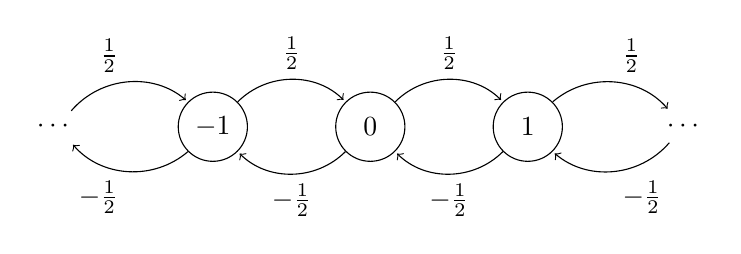
\begin{tikzpicture}[shorten >=1pt,node distance=2cm,auto,bend angle=45]
\node[state]          (q_0)                      {$0$};
\node[state]          (q_-1) [left of =q_0] {$-1$};
\node[]          (q_-2) [left of=q_-1] {$\cdots$};
\node[state]          (q_1) [right of=q_0] {$1$};
\node[]          (q_2) [right of=q_1] {$\cdots$};
\path[->]
          (q_-2)  edge [bend left] node        {$\frac{1}{2}$} (q_-1) 
          (q_-1)  edge [bend left] node        {$\frac{1}{2}$} (q_0) 
          (q_0)   edge [bend left] node        {$\frac{1}{2}$} (q_1) 
          (q_1)   edge [bend left] node        {$\frac{1}{2}$} (q_2)
          (q_2)  edge [bend left] node        {$-\frac{1}{2}$} (q_1) 
          (q_1)  edge [bend left] node        {$-\frac{1}{2}$} (q_0) 
          (q_0)   edge [bend left] node        {$-\frac{1}{2}$} (q_-1) 
          (q_-1)   edge [bend left] node        {$-\frac{1}{2}$} (q_-2);
\end{tikzpicture}
\caption{An automaton}
\label{automaton}
\end{figure}
With that in mind, the $(i,j)$th element of $M^n$ is the number of ways to take a path from $j$ to $i$ in $n$ steps but counting with the given weight.
So
\[
(M^n)_{ij} = \sum_{P:\mbox{$n$ step paths $j\rightarrow i$}} (-1)^{L(P)}\Big(\frac{1}{2}\Big)^n
\]
where I define $L(P), R(P)$ and $n(P)$ to be the number of left steps, right steps and steps respectively in the path $P$.
We have
\begin{align*}
R+L &= n \\
R-L &= i-j \\
\end{align*}
and so also
\[
n = 2L+i-j 
\]
The terms in $e^{aM}$ sum over all paths of any length, but with paths of length $n$ additionally weighted by $\frac{a^n}{n!}$.
This gives us
\[
(e^{aM})_{ij} = \sum_{P:\mbox{paths }j\rightarrow i} \frac{1}{n(P)!}(-1)^{L(P)} (\frac{a}{2})^{n(P)}
\]
There are $\binom{n}{L}=\binom{j-i+2L}{L}$ ways to pick a path with $n$ steps that moves left $L$ times.
So we have
\[
(e^{aM})_{ij} = \sum_{L=0}^\infty\frac{(-1)^{j-i+L}}{L!(j-i+L)!}(\frac{a}{2})^{j-i+2L}
\]
Performing the matrix multiplication gives
\[
b_i(x+a) = \sum_{j=-\infty}^\infty\sum_{L=0}^\infty\frac{(-1)^{j-i+L}}{L!(j-i+L)!}(\frac{a}{2})^{j-i+2L} b_j(x)
\]
Any $(b_i)$ that satisfies this property will satisfy Equations~(\ref{sum}) and (\ref{deriv}).
Just about the simplest thing we could pick for $b_i(x)$ is the sequence with one non-zero element at $x=0$.
So let's define $J_i$ to be the family of Bessel type with $J_i(0)=\delta_{i0}$ giving us
\[
J_i(a) = \sum_{L=0}^\infty\frac{(-1)^{-i+L}}{L!(-i+L)!}(\frac{a}{2})^{-i+2L}.
\]
(Cf. AS-9.1.10)
%There's another way to sum over these weighted paths.

With this definition, we get
\[
e^{aM} = 
M= \begin{pmatrix*}[c]
\ddots & &   &    &   &   &      \iddots  \\
 & J_1(a) & J_0(a) & J_{-1}(a) & J_{-2}(a)  & J_{-3}(a)  &        \\
 & J_2(a)  & J_1(a) & \mathcircled{J_0(a)} & J_{-1}(a) & J_{-2}(a)  &        \\
       & J_3(a)  & J_2(a)  & J_1(a) & J_0(a) & J_{-1}(a) & \\
   \iddots    &   &   &   &   &  & \ddots \\
\end{pmatrix*}.
\]

Note that the addition rule for exponentials now gives us an addition rule for bessel functions.
\[
e^{aM}e^{bM} = e^{(a+b)M}
\]
and so
\[
J_i(x+y) = \sum_{k=-\infty}^\infty J_{k-i}(x)J_{i}(y)
\]
(Cf. AS-9.1.75)
More generally, for any family of functions of Bessel type we have
\[
b_i(x+y) = \sum_{k=-\infty}^\infty J_{k-i}(x)b_{i}(y)
\]

We can think of this as group theoretical. The matrix $e^{aM}$ represents translation by $a$ in one dimension and the addition law is the multiplication in this group.
But this is just a representation of the group of the one dimensional group of translations in one dimension.
We need to return to the three dimensional group of Euclidean motions of the two dimensional plane.

\section{Translations in two dimensions}
We can mimic what we did above in two dimensions.
From (\ref{sum3}) and (\ref{sum4}) we have
\[
\begin{pmatrix}
\vdots \\
\frac{\partial f_{-1}(x,y)}{\partial x} \\
\mathcircled{\frac{\partial f_0(x,y)}{\partial x}} \\
\frac{\partial f_1(x,y)}{\partial x} \\
\vdots \\
\end{pmatrix}
=
M
\begin{pmatrix}
\vdots \\
f_{-1}(x,y) \\
\mathcircled{f_0(x,y)} \\
f_1(x,y) \\
\vdots \\
\end{pmatrix}
\]
and
\[
\begin{pmatrix}
\vdots \\
\frac{\partial f_{-1}(x,y)}{\partial y} \\
\mathcircled{\frac{\partial f_0(x,y)}{\partial y}} \\
\frac{\partial f_1(x,y)}{\partial y} \\
\vdots \\
\end{pmatrix}
=
N
\begin{pmatrix}
\vdots \\
f_{-1}(x,y) \\
\mathcircled{f_0(x,y)} \\
f_1(x,y) \\
\vdots \\
\end{pmatrix}
\]
where
\[
N=\frac{i}{2}
\begin{pmatrix*}[c]
\ddots & \ddots &   &    &   &   &        \\
\ddots & 1 & 0 & 1 &   &   &        \\
       &   & 1 & \mathcircled{0} & 1 &   &        \\
       &   &   & 1 & 0 & 1 & \ddots \\
       &   &   &   &   & \ddots & \ddots \\
\end{pmatrix*}.
\]
Let's call any family of functions $(f_i)$ satisfying these equations a \textit{2-dimensional family of Bessel type}.

If, as usual, we let $z=x+iy$ then the action of translation by $(x,y)$ on $(\ldots,f_{-1}(x,y),f_0(x,y),f_1(x,y),\ldots)$ is given by $e^{P(z)}$ where
\[
P(z) = \frac{1}{2}
\begin{pmatrix*}[c]
\ddots & \ddots &   &    &   &   &        \\
\ddots & \bar{z} & 0 & -z &   &   &        \\
       &   & \bar{z} & \mathcircled{0} & -z &   &        \\
       &   &   & \bar{z} & 0 & -z & \ddots \\
       &   &   &   &   & \ddots & \ddots \\
\end{pmatrix*}.
\]

Just like before, we can view this as a state transition matrix for the automaton in Figure~\ref{automaton2}.

\begin{figure}
\centering
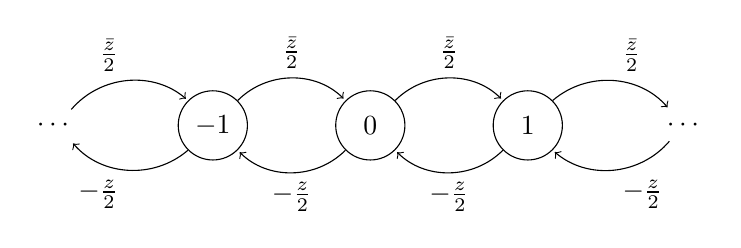
\begin{tikzpicture}[shorten >=1pt,node distance=2cm,auto,bend angle=45]
\node[state]          (q_0)                      {$0$};
\node[state]          (q_-1) [left of =q_0] {$-1$};
\node[]          (q_-2) [left of=q_-1] {$\cdots$};
\node[state]          (q_1) [right of=q_0] {$1$};
\node[]          (q_2) [right of=q_1] {$\cdots$};
\path[->]
          (q_-2)  edge [bend left] node        {$\frac{\bar{z}}{2}$} (q_-1) 
          (q_-1)  edge [bend left] node        {$\frac{\bar{z}}{2}$} (q_0) 
          (q_0)   edge [bend left] node        {$\frac{\bar{z}}{2}$} (q_1) 
          (q_1)   edge [bend left] node        {$\frac{\bar{z}}{2}$} (q_2)
          (q_2)  edge [bend left] node        {$-\frac{z}{2}$} (q_1) 
          (q_1)  edge [bend left] node        {$-\frac{z}{2}$} (q_0) 
          (q_0)   edge [bend left] node        {$-\frac{z}{2}$} (q_-1) 
          (q_-1)   edge [bend left] node        {$-\frac{z}{2}$} (q_-2);
\end{tikzpicture}
\caption{An automaton}
\label{automaton2}
\end{figure}

We can repeat the counting argument.
Let $z=re^{i\theta}$ as usual.
Then if there are $L$ steps left and $R$ steps right then we have a weight of
\[
(-re^{-i\theta})^L(re^{i\theta})^R=r^n(-1)^Le^{i\theta(i-j)}.
\]
It's exactly like before except that each weight is now twisted by $e^{i(i-j)\theta}$.
So the $(i,j)$-th element of $e^{P(z)}$ is given by
\begin{align*}
(e^{aM})_{ij} &= \sum_{L=0}^\infty\frac{(-1)^{j-i+L}}{L!(j-i+L)!}(\frac{r}{2})^{j-i+2L}e^{i(i-j)\theta}\\
              & = J_{i-j}(r)e^{i(i-j)\theta}
\end{align*}

\section{The complete representation of $E(2)$}
So for families of two-dimensional functions of Bessel type we have rotations given by the matrix
\[
R(\phi) = \begin{pmatrix*}[c]
\ddots & \ddots &   &    &   &   &        \\
\ddots & 0 & e^{-i\phi} & 0   &   &        \\
       &   & 0 & \mathcircled{1} & 0 &   &        \\
       &   &   & 0 & e^{i\phi} & 0 & \ddots \\
       &   &   &   &   & \ddots & \ddots \\
\end{pmatrix*}.
\]
and translations given by
\[
T(x,y)= \begin{pmatrix*}[c]
\ddots & &   &    &   &   &      \iddots  \\
 & J_1(r)e^{i\theta} & J_0(r) & J_{-1}(r)e^{-i\theta} & J_{-2}(r)e^{-2i\theta}  & J_{-3}(r)e^{-3i\theta}  &        \\
 & J_2(r)e^{2i\theta}  & J_1(r)e^{i\theta} & \mathcircled{J_0(r)} & J_{-1}(r)e^{-i\theta} & J_{-2}(r)e^{-2i\theta}  &        \\
       & J_3(r)e^{3i\theta}  & J_2(r)e^{2i\theta}  & J_1(r)e^{i\theta} & J_0(r) & J_{-1}(r)e^{-i\theta} & \\
   \iddots    &   &   &   &   &  & \ddots \\
\end{pmatrix*}.
\]

The group law $T(x,y)T(x',y')=T(x+x',y+y')$ should give us another addition formula.
Graf's addition theorem AS-9.1.79.

%When expanding $(t+t^{-1})^n$, the coefficient of $t^m$ is the number of paths with $n$ steps that end up $m$ positions to the right.
%Similarly the coefficient of $t^m$ in $(t-t^{-1})^n$ is the weighted count with weight equal to $(-1)^{\mbox{$\#$ of right steps in path}}$.
%The coefficient
%\[
%e^{a(t-t^{-1})/2}
%\]

\end{document}
